%-------------------------------------------------------------------------------

% This file is part of Code_Saturne, a general-purpose CFD tool.
%
% Copyright (C) 1998-2011 EDF S.A.
%
% This program is free software; you can redistribute it and/or modify it under
% the terms of the GNU General Public License as published by the Free Software
% Foundation; either version 2 of the License, or (at your option) any later
% version.
%
% This program is distributed in the hope that it will be useful, but WITHOUT
% ANY WARRANTY; without even the implied warranty of MERCHANTABILITY or FITNESS
% FOR A PARTICULAR PURPOSE.  See the GNU General Public License for more
% details.
%
% You should have received a copy of the GNU General Public License along with
% this program; if not, write to the Free Software Foundation, Inc., 51 Franklin
% Street, Fifth Floor, Boston, MA 02110-1301, USA.

%-------------------------------------------------------------------------------

%-------------------------------------------------------------------------------
\section{Introduction}

Within the framework of the finite volume approach, the equations are
integrated over each cell of the mesh (or "control volume" $\Omega_i$). 
\nomenclature[gomegai]{$\Omega_i$}{the cell $i$}
This section is limited to a brief description of the way the terms appearing in
the equations are integrated. Specific attention is devoted to the
calculation of gradients, since it is a major characteristic of the
co-located finite volume method (all the variables are associated with the
same point, namely the cell centre\footnote{%
The centre of a cell is a geometric point associated with the cell and
located preferably inside the cell. Nevertheless, the word "centre" shall
not be taken literally,
%The use of the word "centre" is not absolutely correct,
especially in the case of polyhedral cells that do not have a regular shape.}%
).

The terms of \textbf{order 0} (\emph{i.e.} the terms that are not a space
derivative) are integrated to introduce their average over the cell. For
example, $\rho g$ becomes $|\Omega _{i}|\rho_{i}\,g$. 
\nomenclature[gomegaiv]{$|\Omega_i|$}{volume of the cell $i$ \nomunit{$m^{3}$}}
In this expression, $|\Omega _{i}|$ is the volume of cell $\Omega _{i}$ and 
$\rho_{i}$ denotes the average of $\rho $ over the control volume
(the cell) $\Omega _{i}$. When
``reconstructions'' (in fact Taylor series) are required to reach a higher
order in space, the average value $\rho_{i}$ is assumed to be associated
with the centre $I$ of $\Omega _{i}$.
\nomenclature[riu]{$I$}{center of $\Omega_i$}

The ``divergence'' terms (or ``flux'' terms, or again ``conservative''
terms) are integrated using the Green relation to introduce cell faces
values (and so, ``fluxes'' appear naturally). For example, a term such as 
$\dive \left(p \tens{1}\right)$ becomes\footnote{%
If the cell $i$ is at the domain boundary, the sum becomes 
$\sum\limits_{j\in \Neigh{i}}p_{ij}S_{ij}+\sum\limits_{b \in \Bound{i}
}p_{b}S_{b}$, 
with $b$ referring to the faces
of the cell $i$ which are at the domain boundary.} 
$\sum\limits_{j \in \Neigh{i}} p_{ij}S_{ij}$.
In this expression, $p_{ij}$
is the average of $p$ on the interface between the neighbouring cells $i$
and $j$. The summation is carried out for $j\in \Neigh{i}$, that is, all
cells in the neighbourhood of $\Omega_{i}$ thus sharing a cell face with
it. The value $p_{ij}$ is
\nomenclature[rpij]{$p_{ij}$}{average of the pressure field on the interface between the neighbouring cells $i$ and $j$ \nomunit{$Pa$}}
assumed to be associated with the centre $F$
\nomenclature[rfu]{$F$}{center of the face $ij$ between cells $i$ and $j$}
 of the face $ij$ when
``reconstructions'' are needed to reach a higher order in space.

The precision of the value $p_{ij}$ determines the precision of the
calculation of $\dive \left(p \tens{1}\right)$. For $p_{ij}$, it is possible to take a non-centred
and non-interpolated value (upwind scheme for convection) or a linear
interpolation between the values at the centres I and J of the neighbouring
cells. Both methods are relatively straighforward but may lack consistence
and precision for arbitrary meshes (and in particular on non-orthogonal
meshes). A higher order in space may be reached if reconstruction techniques
are used. The idea is to compute the value for $p_{ij}$ more precisely: to
do so, $p$ is interpolated at $F_{ij}$ (the centre of the face) using the
values for $p$ at $I$ and $J$ and the gradients of $p$ calculated at $I$ and $J$.
The reader will notice that it is precisely the calculation of the space
derivatives\footnote{%
The first derivatives in space are required to obtain $\dive \left(p \tens{1}\right)$ in each cell.}
of $p$ that motivated the need for a good interpolation of $p$ at $F_{ij}$.
Hence, the computation of the space derivatives of $p$ requires to solve a
system: this is done in an iterative manner (see \S~\ref{sec:space_discretization_it_grad} and \S~\ref{ap:gradrc}).

Doing so allows to calculate the \textbf{``cell gradient''} of the variables.
It is important to keep in mind that the ``cell gradient'' of a given variable
represents the gradient of the variable in the cell and that it is obtained
from the values of the variable interpolated at the cell faces.

Similarly, the terms written as \textbf{``divergence of gradient''} are
integrated to introduce face values. One has to calculate the gradient at
each face (or ``face gradient'') in the direction normal to the face. This
concept of ``face gradient'' is extremely important. The ``face gradient''
normal to a face can be easily calculated with just the values at the
centres of the two cells that share the face (points $I$ and $J$ on 
\figurename~\ref{fig:sketch_internal_external_faces}),%Base_Introd_fig_geom}), 
but this method is limited to orthogonal meshes.
% fa modification : reconstruction is compulsory for consistence
For consistence and to reach a higher order in space, the values of the
variables at points $I'$ and $J'$ have to be used. These are calculated by a
Taylor series from the values at $I$ and $J$ and from the ``cell gradient''
previously determined.

\begin{figure}[t]
\centering
\mbox{
\subfigure[Internal face]{
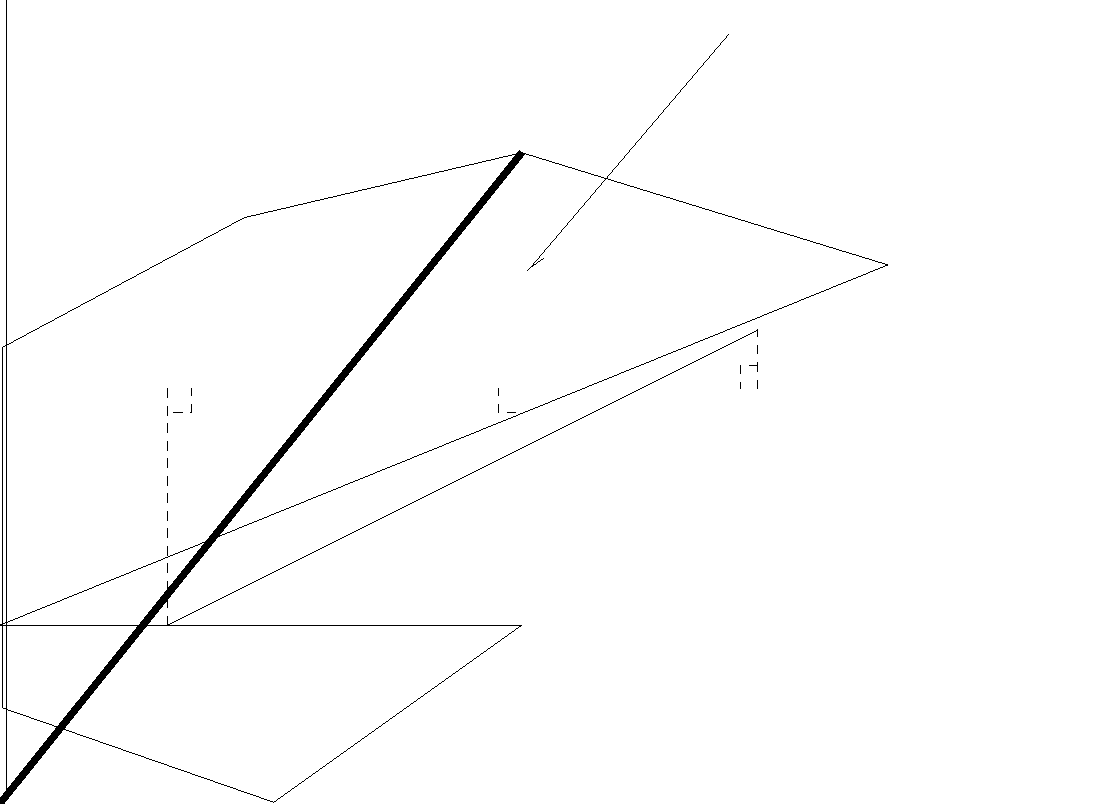
\includegraphics[width=0.45 \textwidth]{facette}
} \,
\subfigure[Boundary face]{
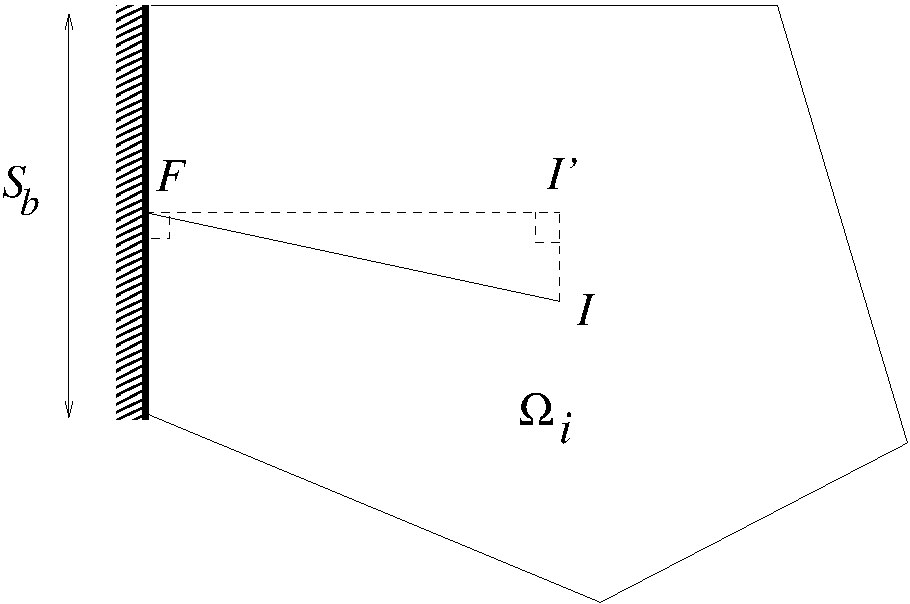
\includegraphics[width=0.45 \textwidth]{facebord}
}
}%end mbox
\caption{Sketch of the geometric entities.}
\label{fig:sketch_internal_external_faces}
\end{figure}

%-------------------------------------------------------------------------------
\section{Gradient calculation}
Work in progress.
\subsection{Standard method}\label{sec:space_discretization_it_grad}
Work in progress.
\subsection{Least-square method}
Work in progress.